\documentclass[./main]{subfiles}
\begin{document}

\Chapter{パズルのコーナー(まどれ〜ぬ)} 
\Section{てこのパズル}
\noindent 〈ルール〉指定された重さのおもりを1つずつ配置して、すべての棒が水平に釣り合うようにします。棒と糸の重さ\\
 は、無視できるものとします。\\
 ※棒が釣り合う条件は、支点の左右で(重さ)×(距離)の和が等しくなることです。\\[15pt]
              例題                  例題の答え
\begin{center}
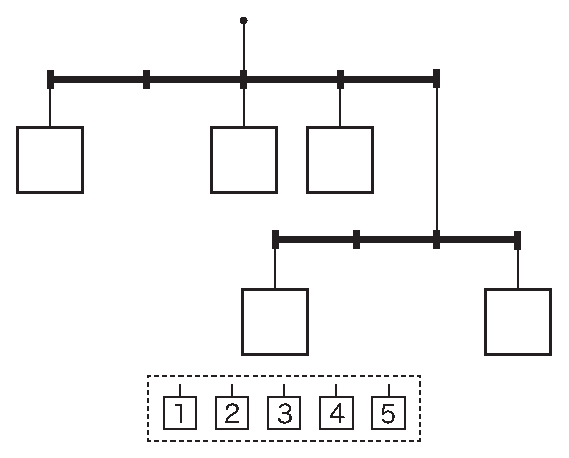
\includegraphics[scale=0.6]{morikawa_image/morikawa_puzzle_inst_p.eps}     
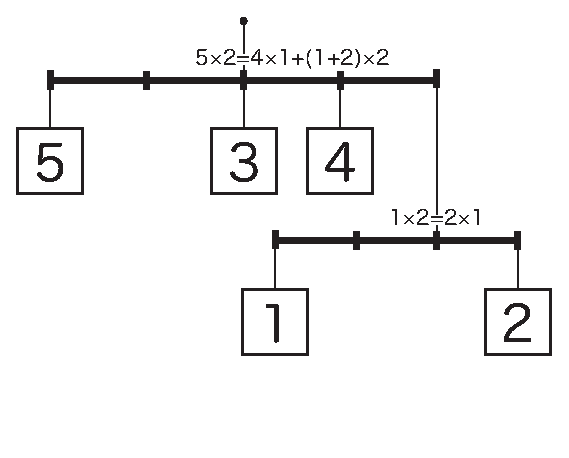
\includegraphics[scale=0.6]{morikawa_image/morikawa_puzzle_inst_a.eps}
\end{center}
1.
\begin{center}
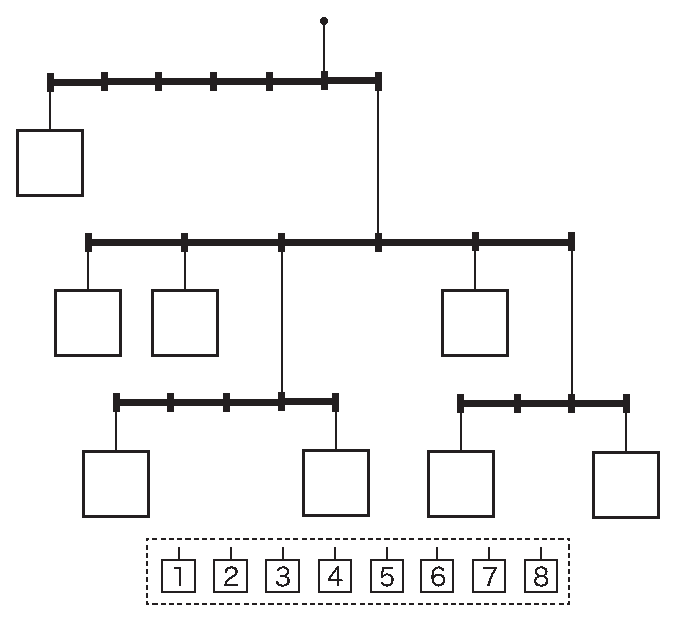
\includegraphics[scale=0.6]{morikawa_image/morikawa_puzzle_1.eps}
\end{center}
2.
\begin{center}
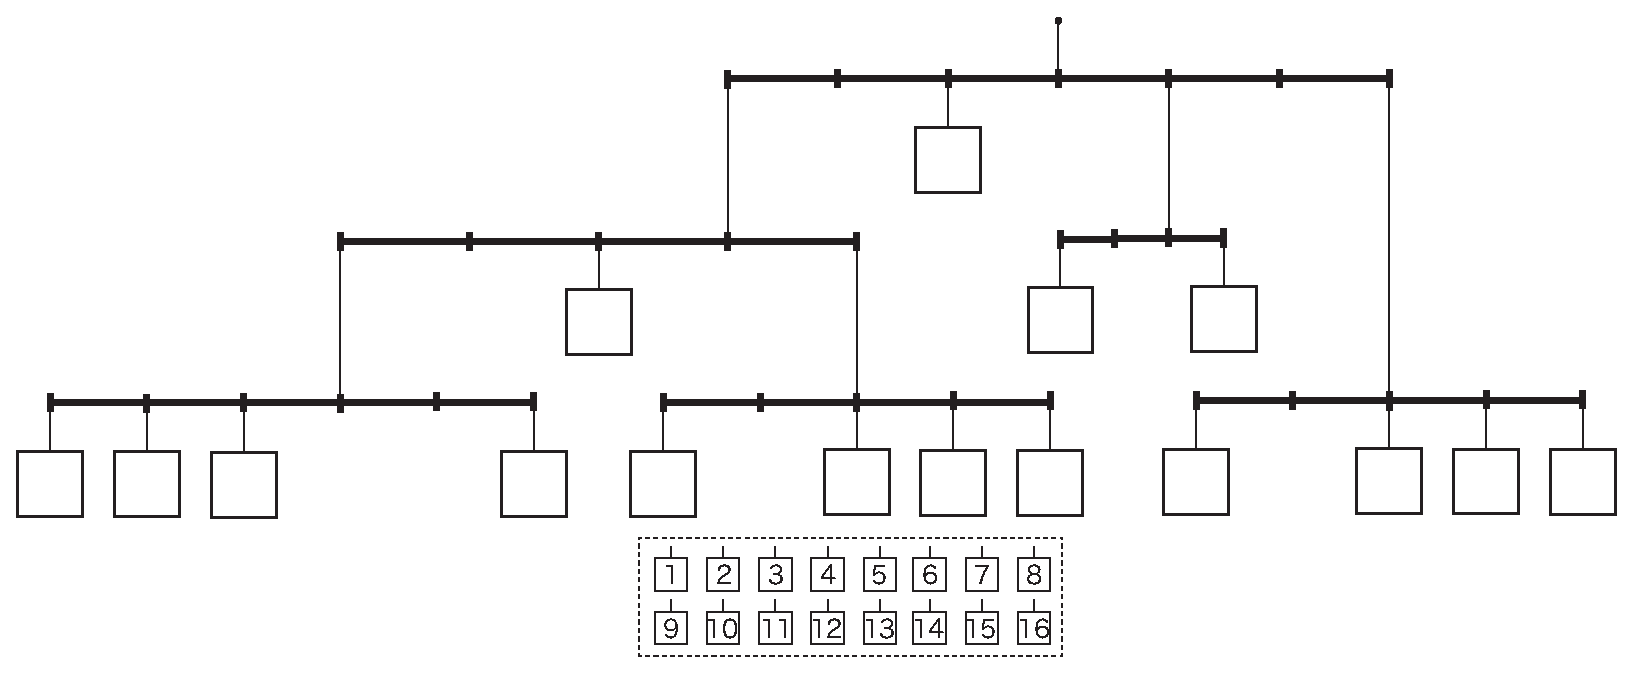
\includegraphics[scale=0.6]{morikawa_image/morikawa_puzzle_2.eps}
\end{center}
\end{document}

%\begin{thebibliography}{9}
%\item Hull, J. C. (2014), Options, Futures, and Other Derivatives, 9th edition (Upper Saddle River, NJ: Prentice Hall).
%\end{thebibliography}
